\documentclass[a4paper,12pt,fleqn]{article}%fleqn pour aligner les equations à gauche
\usepackage{../Styles/Cours}


\newcommand{\chnum}{Chapitre 1}
\newcommand{\chtitle}{Transformation acide-base et pH}
\newcommand{\dtype}{Cours}

\begin{document}
Bonjour !

\begin{figure}
	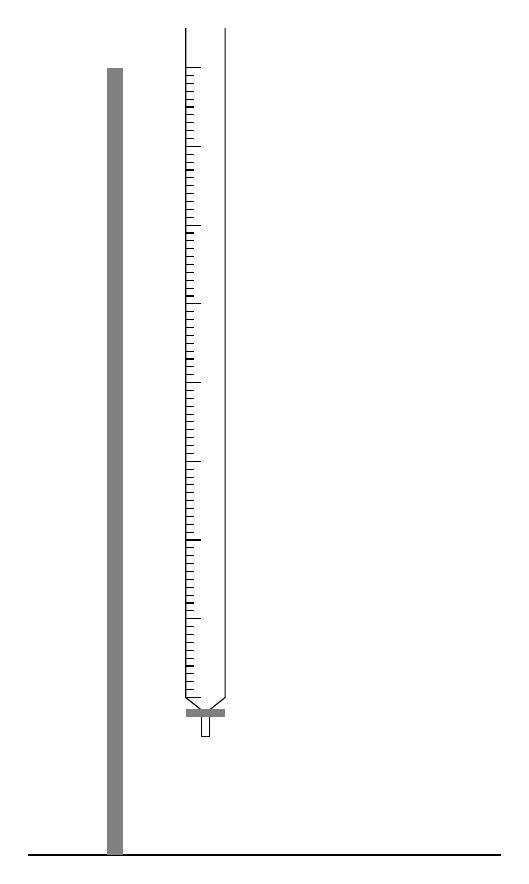
\begin{tikzpicture}
		\draw (0,0) -- (6,0);
		\fill[gray] (1,0) -- (1,10) -- (1.2,10)-- (1.2,0) -- cycle ;
		\draw (2,10.5) -- (2,2)--(2.25,1.8)--(2.5,2)--(2.5,10.5);
		\draw (2.2,1.8)--(2.2,1.5)--(2.3,1.5)--(2.3,1.8);
		\draw[line width = .1cm,color=gray] (2,1.8)--(2.5,1.8);
		
		\foreach \k in {2,3,4,5,6,7,8,9,10}{
			\draw (2,\k )--(2.2,\k );
			}

		\foreach \k in {2.1,2.2,...,10}{
			\draw (2,\k )--(2.1,\k );
			}
	\end{tikzpicture}
\end{figure}
\end{document}

